In this Section we present some experimental results on the case study presented in Section \ref{sec:case_study}. We want to check if \emph{Property 1} is verified on the program of Figure \ref{lst:casestudy} and, in particular, we want to know which subset of starting values brings to verify it.
We implemented our analysis in the \FSharp\ language with Visual Studio 2012. We ran the analysis on an Intel Core i5 CPU 1.60 GHz with 4 GB of RAM, running Windows 8 and the \FSharp\ runtime 4.0 under .NET 4.0. 

We set the initial widths associated to all variables to $100.0$ and the minimum width allowed to $5.0$. As for \emph{Property 1}, we set $T = 5$, i.e., we want to verify if the ball is surely out of the screen within $5$ seconds from its generation. Since $dt=0.05$, a simulation during $5$ seconds corresponds to $5/0.05 = 100$ iterations of the \statement{while} loop. To verify this property, we apply trace partitioning \cite{MR05} to track one abstract state per loop iteration until the 100-th iteration (we do not need to track precise information after the 100th iteration). The position which corresponds to the exiting from the screen is $100.0$: if after $100$ iterations the position \statement{px} is surely greater than $100.0$, then \emph{Property 1} is verified. The whole of these values (starting variables values and widths, minimum width allowed, number of iterations, position to reach) make up our \emph{standard workbench data}. We will experiment to study how efficiency and precision change when modifying some parameters of the analysis.
%, and for each test we will specify only the values which are different with respect to the standard workbench data.
%We will start by running the analysis on the standard workbench data, and then we will experiment by changing one value at a time to study how the efficiency and precision change\footnote{}. 

%For example, we will start by showing how precision and performance are affected by changing the minimum width allowed. After that, we will concentrate on the horizontal velocity variable and we will show how we can use our analysis as a form of \textquotedblleft assisted debugging\textquotedblright\ to understand which starting values of a variable bring to verify the property and which not. 

For each test, the analysis returns three sets of starting hypercubes: the initial values of the variables which satisfy the property (\textit{yes} set), which surely do not satisfy the property (\textit{no} set), and which may or not satisfy the property (\textit{maybe} set). To make the results more immediate and clearer, we computed for each \emph{yes} and \emph{no} set the corresponding volume covered in the space by their hypercubes. We also consider the \emph{total} volume of the variable space, i.e., the volume covered by all possible values with which the program variables are initialized. In the case of the standard workbench data, the \emph{total} volume is $10.0 \times 50.0 \times 60.0 \times 5.0 = 150000$. Dividing the sum of \emph{yes} and \emph{no} volumes by the \emph{total} volume, we obtain the percentage of the cases for which the analysis gives a definite answer. We will call this percentage the precision of the analysis. 

%Note that the \emph{total} volume refers to the initial variable space, i.e., to the space defined by the intervals assigned to the variables at the beginning of the program. The \emph{yes}, \emph{maybe}, and \emph{no} volumes refer to the same space, since they are defined in terms of \emph{starting} hypercubes. These volumes are all finite, since we suppose that all the variables are initialized by a bound interval, and this is always the case in Computer Games Software.

\subsubsection{Varying the minimum width allowed}
First of all, we run the analysis modifying the \emph{minimum width allowed} (MWA) parameter and we reported the results of these tests in Table \ref{table:minWidthAllowed}. We can clearly see the trade-off between performance and precision. %that the performance decreases when we set small widths, and it is instead very good on bigger ones. On the other hand, by decreasing the MWA we also gain more precision. 

\vspace{-15pt}
\begin{table}[ht]
\scriptsize
\caption{Varying the minimum width allowed (MWA)}
\centering 
\begin{tabular}{| c | c | c | c |}
\hline
MWA & Time (sec.) & \emph{yes+no} volume & Precision \\ \hline
3 & 530 & 131934 & 88\%  \\ %\hline 
5 & 77 & 99219 & 66\%  \\ %\hline 
12 & 11 & 40625 & 27\%  \\ %\hline 
24 & 1 & 25000 & 17\% \\ %\hline 
45 & 0.2 & 0 & 0\% \\ \hline 
\end{tabular}
\label{table:minWidthAllowed} 
\end{table}
\vspace{-30pt}

%\begin{figure}
%\begin{center}
%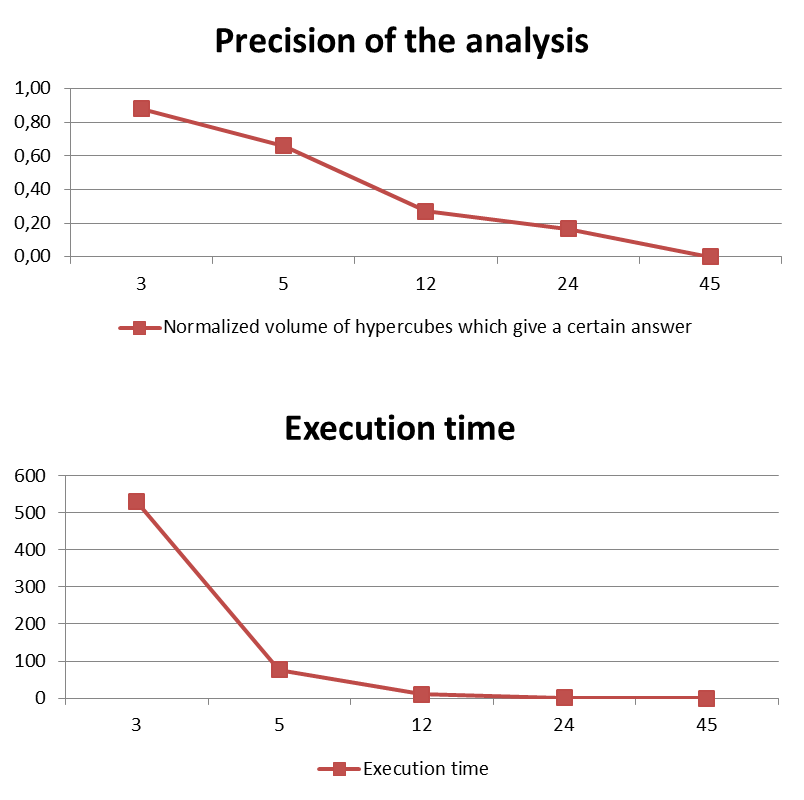
\includegraphics[scale=0.6]{Pics/varyingMWA.png}
%\caption{Varying the minimum width allowed - Plots}
%\label{fig:minWidthAllowed}
%\end{center}
%\end{figure}

%From these results,  For instance, when MWA = 45 we do not have any certain answer, while with MWA = 3 the certain answers cover the 88\% of the volume space, a quite precise result. 

\subsubsection{Finding appropriate starting values}

In Table \ref{table:velocityX} we reported the results of a series of successive tests obtained by changing the horizontal velocity of the ball (\statement{vx}). In particular, we made up a series of tests simulating the behavior of a developer using our analysis to debug his code. Let us suppose that we wrongly inserted a starting interval of negative values (between -120 and 0) for the horizontal velocity. The first test (\# 1) shows us that the program does not work correctly, since the \emph{no} volume is 100\%. Also, to give this answer, the analysis is very quick because a low MWA (45) suffices. After that, we try (test \# 2) with very high positive velocities (between 60 and 120) and we obtain (also very quickly) a 100\% of positive answer: we know for sure that with these velocities the program works correctly. Now it remains to verify what happens with velocities between 0 and 60, and we try this in test \# 3, where we decrease the MWA because we need more precision (the results with greater MWA were presented by the previous Section). Some values of \statement{vx} (i.e., $\geq 31.25$) ensure that the property is verified, some other values (i.e., $\leq 12.5$) ensure that the property is not verified, but the ones in between are uncertain. Tests \# 4 and \# 5 are just double checks.
%To do a double check about this data, we execute also tests \# 4 and \# 5, where we keep, respectively, only the low (between 0 and 15) and the high (between 30 and 60) values: in both cases the analysis is fairly quick in confirming the 100\% \emph{no} and 100\% \emph{yes}. 
So we try with a smaller MWA (3) in test \# 6 on the interval $[15..30]$: about a quarter of the starting values produces \emph{yes} and another quarter produces \emph{no}. The \emph{no} derives from low values (smaller than 18) and we confirm this in test \# 7. %, where (with a MWA of 5 and quick execution time) we obtain a 100\% of \emph{no} answers. 
As for medium-high values, test \# 6 shows that, with a velocity greater than 25, the answer is \emph{almost} always \emph{yes}. It is not always yes because, with this range of velocities, the values of other variables become important to verify the property. Test \# 8, in fact, shows us that velocities within 25 and 30 produce an 82\% of \emph{yes}, but a 18\% of \emph{maybe} remains. Finally, in test \# 9 we modify also other two variables (with values chosen looking at the results from test \# 6 and \# 8)
%: in particular, we set the horizontal position (\statement{px}) between 5 and 10, and the vertical position (\statement{py}) between 40 and 50. 
and, with such values, the answers are 100\% \emph{yes}. 

After these tests, the developer of the case study is sure that horizontal velocities below 18 will certainly not make the program work. On the other hand, values greater than 30 certainly make the program work. For values between 25 and 30, other variable values must be changed (\statement{px} and \statement{py}) to make the program work correctly. Making some other tests, we could also explore what happens with values between 18 and 25. 

\begin{table}[ht]
\scriptsize
\caption{Varying the horizontal velocity (\statement{vx})}
\centering 
\begin{tabular}{| l | c | c | c | l | p{5cm} |}
\hline
Test & \statement{vx} interval & MWA & Time (sec) & Answer & Comment \\ \hline
\# 1 & [-120 .. 0] & 45 & 1 & \emph{no} = 100\% & With negative values the answer is always no. \\ \hline 
\# 2 & [60 .. 120] & 45 & 0.2 & \emph{yes} = 100\% & With very high positive values the answer is always yes. \\ \hline 
\# 3 & [0 .. 60] & 5 & 77 & 
$\begin{array}{l}
\emph{yes} = 45\%\\
\emph{no}  = 21\%
\end{array}$ & Uncertainty. High values ($\geq$ 31.25) imply \emph{yes}, low values ($\leq$ 12.5) imply \emph{no}. \\ \hline 
\# 4 & [0 .. 15] & 24 & 0.5 & \emph{no} = 100\% & Double check on low values: answer always no. \\ \hline 
\# 5 & [30 .. 60] & 5 & 30 & \emph{yes} = 100\% & Double check on medium-high values: answer always yes. \\ \hline 
\# 6 & [15 .. 30] & 3 & 526 &
$\begin{array}{l}
\emph{yes} = 27\%\\
\emph{no} = 25\%
\end{array}$ & Uncertainty. Low values ($\leq$ 18) imply \emph{no}, for high values ($\geq$ 25) depends also on other variables. \\ \hline 
\# 7 & [15 .. 18] & 5 & 7 & \emph{no} = 100\% & Double check on medium-low values: answer always no. \\ \hline 
\# 8 & [25 .. 30] & 3 & 164 & 
$\begin{array}{l}
\emph{yes} = 82\%\\
\emph{maybe} = 18\%
\end{array}$ & Double check on medium-high values: answer almost always yes. In this case, also values of other variables influence the result. \\ \hline 
\# 9 & [25 .. 30] & 5 & 1 & \emph{yes} = 100\% & Modified also py ([40 .. 50]) and px ([5 .. 10]). Answer always yes. \\ \hline 
\end{tabular}
\label{table:velocityX} 
\end{table}
\vspace{-10pt}

\subsubsection{Discussion}
In this scenario, we ran the analysis by manually changing the initial values of program variables. Notice that this process could be automatized. 
%In particular, instead of providing a program that initializes all the variables, and checking if a given property holds, a user could give only the \statement{while} loop that performs the physics simulation, and then try wide ranges of initial values for the variables. This will obviously lead to an analysis that, even with large widths, could quickly give definite answers for a wide part of the given starting intervals. 
This process can be highly interactive, since the tool could show to the user even partial results while it is automatically improving the precision by adopting narrower intervals on the \emph{maybe} portion as described by Algorithm \ref{alg:widthAdjusting}. In this way, the user could iterate the process until it finds suitable initial values.

The execution times obtained so far underline that the analysis is efficient enough to be the basis of practical tools. Moreover, the analysis could be parallelized by running in parallel the computation of the semantics for each initial hypercube: exploiting several cores or even running the analysis in the cloud, we could further improve the efficiency of the overall analysis.
%. In this way, when we choose a narrow width, we could exploit several cores or even run the analysis in the cloud, thus improving the efficiency of the overall analysis.

